Pour chaque question, recopier sur la copie son numéro et la réponse correspondante.

Pour cette partie, aucune justification n'est demandée.

Pour les questions à choix multiple, une seule réponse est exacte.

\subsection*{Question 1}

Quelle est l'abscisse du point A ?

%Début Tikz
\begin{center}
\begin{tikzpicture}[x=0.75cm,line cap=round, line join=round]
	\draw[line width=1.2pt,-{Stealth}] (-2.8,0) -- (13.2,0);
	\foreach \i in {-2,...,12} \draw[line width=1pt] (\i,-0.1) -- (\i,0.1);
	\node[below=2pt] at (0,0) {4,6};
	\node[below=2pt] at (10,0) {4,7};
	\draw[line width=1pt,red] (8,0) ++(2pt,2pt)--++(-4pt,-4pt) ++(0,4pt)--++(4pt,-4pt);
	\node[above=2pt] at (8,0) {A};
\end{tikzpicture}
\end{center}
%Fin Tikz

\subsection*{Question 2}

Quelle expression est égale à $4x+6x$ ?

\begin{center}
\begin{tblr}{*{4}{|X[c]}|}\hline
	\textbf{A.} $10x^2$ & \textbf{B.} $24x^2$ & \textbf{C.} $10x$ & \textbf{D.} $24x$ \\
	\hline
\end{tblr}
\end{center}

\subsection*{Question 3}

On tire au hasard une boule dans un sac et on sait que la probabilité d'obtenir une boule rouge est 0,4.

Quelle est la probabilité de ne pas obtenir une boule rouge ?

\subsection*{Question 4}

Une voiture part à 7~h 10~min. Le trajet dure 53~min.

À quelle heure arrive-t-elle ?

\subsection*{Question 5}

Le prix d'un objet est de 150~\euro. Il augmente de 10\,\%.

Quel est son nouveau prix ?

\begin{center}
\begin{tblr}{*{4}{|X[c]}|}\hline
	\textbf{A.} 135~\euro & \textbf{B.} 150,10~\euro & \textbf{C.} 160~\euro & \textbf{D.} 165~\euro \\
	\hline
\end{tblr}
\end{center}

\subsection*{Question 6}

Le graphique ci-dessous donne la taille d'une personne en fonction de son âge.

%Début Tikz
\begin{center}
		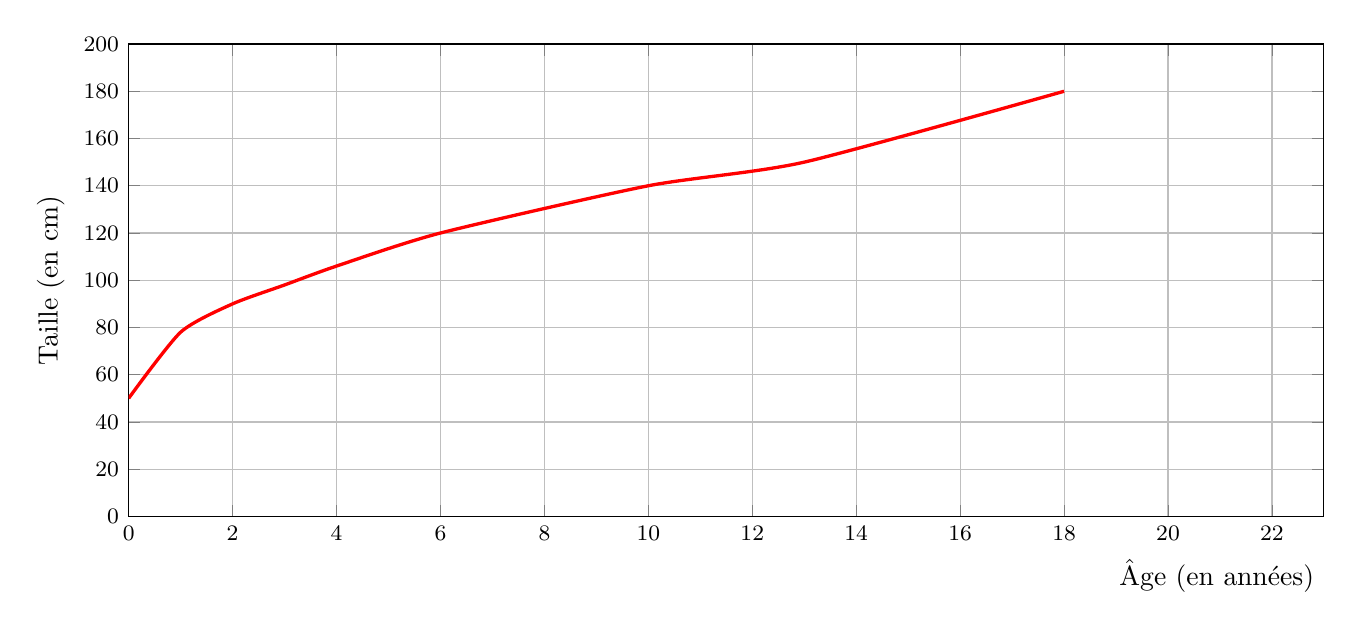
\begin{tikzpicture}%compiler avec pgfplots
			\begin{axis}[/pgf/number format/.cd, use comma,
				xlabel={Âge (en années)},
				xlabel style={
					at={(ticklabel cs:1)},
					anchor=north east},
				ylabel={Taille (en cm)},
				x={6.6mm}, y={0.3mm},
				xmin = 0, xmax = 23,
				ymin = 0, ymax = 200,
				xtick distance=2,
				ytick distance=20,
				tick label style={font=\footnotesize},
				grid=major]
				\addplot [line width=1.2pt,color=red,smooth,tension=0.4] coordinates
					{(0,50) (1,78) (2,90) (3,98) (4,106) (6,120) (10,140) (13,150) (18,180)};
			\end{axis}
		\end{tikzpicture}
\end{center}
%Fin Tikz

À partir de quel âge la taille de cette personne a-t-elle dépassé 140~cm ?

\subsection*{Question 7}

Parmi les nombres ci-dessous, lequel est divisible par 3 ?

\begin{center}
\begin{tblr}{*{4}{|X[c]}|}\hline
	\textbf{A.} 307 & \textbf{B.} 954 & \textbf{C.} \np{1201} & \textbf{D.} \np{22003} \\
	\hline
\end{tblr}
\end{center}

\begin{minipage}{0.52\linewidth}
\subsection*{Question 8}

La figure ci-contre n'est pas représentée en vraie grandeur.

Quelle est la mesure de l'angle $\widehat{\mathrm{BAC}}$ ?

\medskip

\begin{tblr}{*{2}{|X[c]}|}\hline
	\textbf{A.} 80\degres & \textbf{B.} 90\degres \\ \hline
	\textbf{C.} 100\degres & \textbf{D.} 110\degres \\ \hline
\end{tblr}
\end{minipage}\hfill
%Début Tikz
\begin{tikzpicture}[line cap=round, line join=round,baseline={(current bounding box.center)}]
	\coordinate (B) at (0,0);
	\coordinate (C) at (5.5,-0.5);
	\coordinate (A) at (3.3,2.9);
	\draw[line width=1pt,fill=blue!30] (B) -- ($(B)!0.6cm!(C)$) arc[start angle={atan2(-0.5,5.5)}, delta angle=47, radius=0.6cm] -- cycle;
	\draw[line width=1pt,fill=red!30] (C) -- ($(C)!0.6cm!(A)$) arc[start angle={atan2(3.4,-2.2)}, delta angle=53, radius=0.6cm] -- cycle;
	\draw[line width=1.2pt] (A) -- (B) -- (C) -- cycle;
	\node[font=\small] at ($(B)+(22:1.05)$) {47\degres};
	\node[font=\small] at ($(C)+(150:1.1)$) {53\degres};
	\node[above] at (A) {A};
	\node[left] at (B) {B};
	\node[below right] at (C) {C};
\end{tikzpicture}\hfill~
%Fin Tikz

\subsection*{Question 9}

Quel est le résultat de $\dfrac{5}{8} \div \dfrac{8}{9}$ ?

\begin{center}
\begin{tblr}{*{4}{|X[c]}|}\hline
	\textbf{A.~~} $\dfrac{45}{64}$ & \textbf{B.~~} $\dfrac{45}{8}$ & \textbf{C.~~} $\dfrac{40}{72}$ & \textbf{D.~~} $\dfrac{5}{9}$ \\
	\hline
\end{tblr}
\end{center}
